\chapter{Two Applications of Persistent Homology}

Our purpose with thesis is not only to give an introduction to persistent homology in terms of theory, but also display how it can be used with actual real-world data. As such, we illustrate the practical workflow of persistent homology with two different case studies where the analysis of persistent homology serve as our main tool.

In the first case we quantify differences in morphology between different-sized individuals of the bumblebee \textit{Bombus terrestris} by computing the persistent homology of 3D volumes of their corneas. To our knowledge this is the first use of persistent homology in data pertaining to insects, although materials \cite{moon2019, delgadofriedrichs2014}, reconstructions of 3D volumes \cite{gutierrez2012, gutierrez2014} and plants \cite{plants} have been investigated with approaches that are similar in spirit.

In the second case we try to understand the network structure of the striatum, a part of the basal ganglia in the brain. Due to the sheer computational power needed to compute persistent homology for this data our analysis is more of a holistic summary of the resulting simplicial structure rather than focusing solely on persistent homology. Our approach is largely inspired by \cite{reimann}, in which a similar analysis is done but for a different part of the brain.

The application of persistent homology to a data set is not entirely trivial. In order to compute persistent homology we need to construct a persistence complex on the data at hand. This can be done in a multitude of ways, but the basic pipeline can be seen in Figure \ref{pipeline}.

\begin{figure}[h]
  \centering
  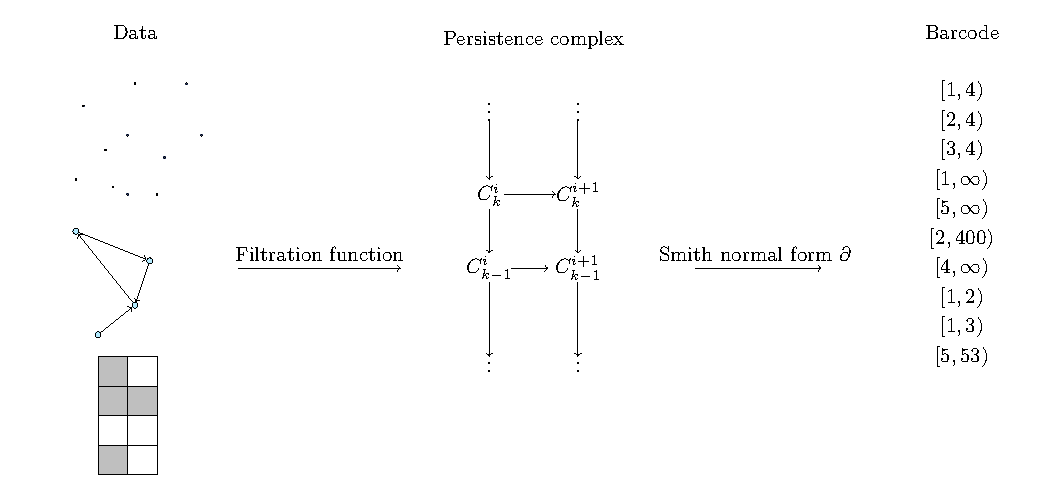
\includegraphics[scale=0.8]{pipeline.pdf}
  \caption{\label{pipeline} The pipeline of computing persistent homology of data.}
\end{figure}

A central part of this pipeline is the formulation of a filtration function that yields a sequence of complex and hence a persistence complex. The filtration provides the translation of data into an algebraic object we can compute persistent homology of. When we analyze results from persistent homology, perhaps by comparing metrics between two barcodes or reading directly of a persistence diagram, the semantic meaning of those results is intimately connected to how the filtration creates the resulting complex. Dually, this means that to formulate the filtration we need to have a strong understanding of the data itself so that our filtration captures essential properties of the data. The complex constructed on the data set is topologically an approximation, but since it is not the ``true'' space in which the data lives care has to be taken so that any conclusions made from the barcode are meaningful.


\section{Corneas of Bombus terrestris}
It has been found that the size of individuals of the species \textit{Bombus terrestris} affects aspects of their visual capabilities \cite{emily}. By applying persistent homology we can investigate whether this difference in size also translates to a difference in persistent homology, and so by proxy a difference in topology. If so, this could serve to strengthen the hypothesis that larger individuals have superior, or at the very least different, visual capabilities than smaller individuals. Persistent homology is a good candidate for this purpose as metrics on persistence diagrams are indifferent to differences in scale but rather measures differences in shape.

Our questions we wish to investigate in this case study are
\begin{enumerate}
  \item Is there a correlation between the size of the bumblebees and their persistent homology?
  \item Can we with persistent homology identify subgroups of bumblebees, and if so are these subgroups related to their size?

\end{enumerate}
\subsection{Data}
The data consists of binary 3-dimensional volumes (see Figure \ref{corneas} for renderings of some of the samples) of the corneas acquired by micro-CT scans of the samples as well as their intertegular width (ITW) described in Table \ref{bees}. The ITW of a bee is known to be an accurate estimator of its size \cite{itw}.

The main focus of the analysis will be on samples from the bumblebee \textit{Bombus terrestris}, but in total there are 20 samples belonging to 8 different species of insects. We use the additional samples from other species to verify our topological findings.

\begin{figure}[h]
  \centering
  \begin{subfigure}{.3 \linewidth}
  \centering
  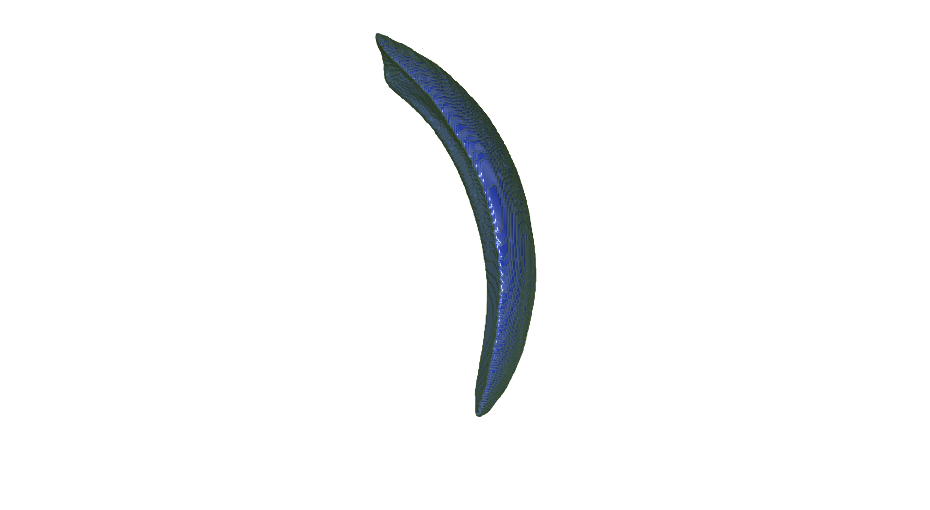
\includegraphics[scale=0.2]{ta60204_cornea.png}
  \caption{TA\_60204}
  \end{subfigure}%
  \begin{subfigure}{.3 \linewidth}
  \centering
  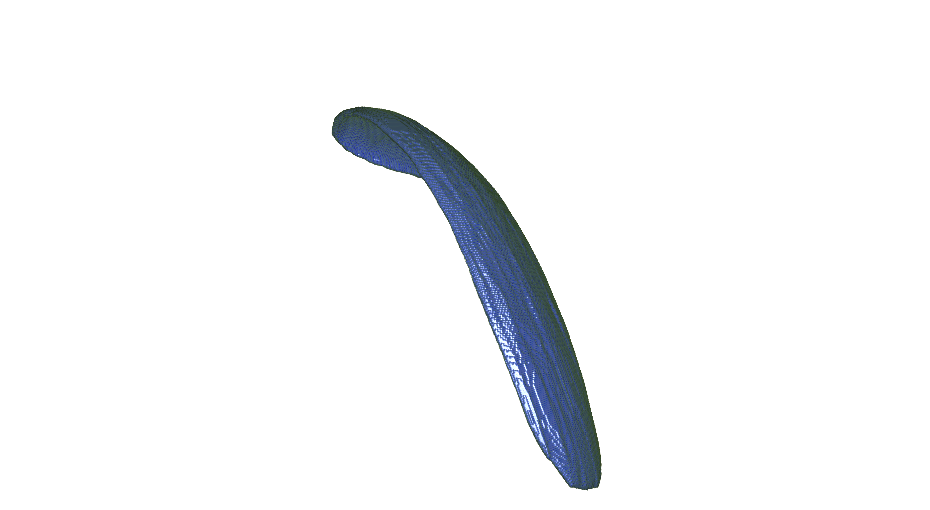
\includegraphics[scale=0.2]{mq60209_cornea.png}
  \caption{MQ\_60209}
  \end{subfigure}%
  \begin{subfigure}{.3 \linewidth}
  \centering
  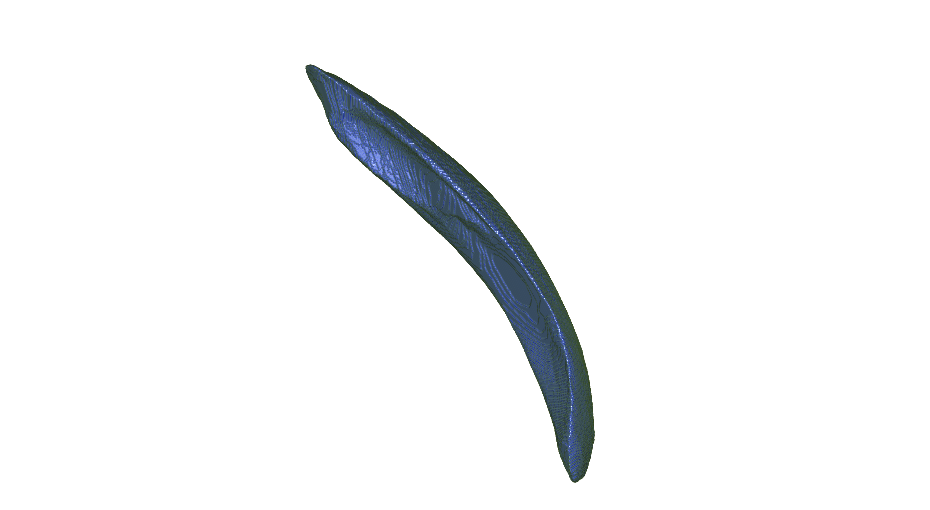
\includegraphics[scale=0.2]{bt77970_cornea.png}
  \caption{BT\_77970}
  \end{subfigure}
  \caption{\label{corneas} Example renderings of cornea volumes.}
\end{figure}
\begin{table}[h]
\begin{center}
\begin{tabular}{*6l}
\toprule
  ID & ITW & Species  \\ \midrule
AM\_60185 & 2.90 & Apis mellifera \\
AM\_60186 & 2.95 & Apis mellifera \\
BT\_77967 & 5.42 & Bombus terrestris \\
BT\_77970 & 4.00 & Bombus terrestris \\
BT\_77971 & 4.02 & Bombus terrestris \\
BT\_77973 & 1.97 & Bombus terrestris \\
BT\_77974 & 2.97 & Bombus terrestris \\
BT\_77976 & 5.47 & Bombus terrestris \\
MB\_60160 & 3.25 & Melipona bicolor \\
MB\_60161 & 3.25 & Melipona bicolor \\
MQ\_60208 & 3.64 & Melipona quadrifasciata \\
MQ\_60209 & 3.64 & Melipona quadrifasciate \\
PR\_60164 & 1.49 & Plebia remota \\
PR\_60206 & 1.49 & Plebia remota \\
TA\_60204 & 1.17 & Tetragonista angustula \\
TA\_78016 & 1.17 & Tetragonista angustula \\
TC\_60166 & 1.94 & Tetragona clavipes \\
TC\_60167 & 1.94 & Tetragona clavipes \\
TS\_60163 & 2.10 & Trigona spinipes \\
TS\_60203 & 2.10 & Trigona spinipes \\
  \bottomrule
\end{tabular}
\caption{Table over the data samples used in the analysis. The ID column gives a unique ID to each sample and the ITW column gives the intertegular width of each sample.}
\label{bees}
\end{center}
\end{table}
\subsection{Methodology}
Since the data we are working with are 3-dimensional volumes a natural choice is to endow it with the structure of a cubical complex. Our strategy is similar to the Vietoris-Rips complex, but instead of working with distances between points we work with adjacent cubes. Each voxel can be considered as a degenerate interval (or vertex) in a cubical complex, where $4$ pairwise adjacent voxels give rise to a square and $8$ pairwise adjacent voxels give rise to a cube.

In order to compute persistent homology we need a filtration which defines subcomplexes of the cubical complex. Since the volumes are binary, we give the volume a bit more structure by giving each voxel the distance to the closest point on the volume's boundary.
\begin{definition}
  Given a subset $Y \subset \mathbb{R}^{n}$ we define the Euclidean Distance Transform, or EDT, as
   \[EDT(x) = \inf_{y \in \partial Y} ||x - y||_2\]
   where $\partial Y$ is the boundary of $Y$.
\end{definition}

Our filtration is a sequence of cubical complexes $K_{i}$ given by including voxels whose EDT is at most $\epsilon_{i}$ as degenerate intervals. Higher dimensional cubes such as edges, squares and geometric cubes are, similarly to the Vietoris-Rips complex, included whenever there is a sufficient amount of pairwise adjacent voxels.

\begin{example}
  To calculate the EDT of the binary image in Figure \ref{edt} we simply calculate the difference vector from a pixel of value $1$ to the closest pixel with value $0$. For example, to get $\sqrt 5$ in the top left corner we need to walk one step in to the left and two steps upwards which translates to the vector $(-1,2)$ which has Euclidean norm $\sqrt{1+4}=\sqrt{5}$. We then compute the filtration of the transformed image, which gives us cubical complexes for each value of $\epsilon$. Since there are five distinct values of the pixels, we find  five subsequent cubical complexes ordered by inclusion.

  \begin{figure}[ht]
    \centering
    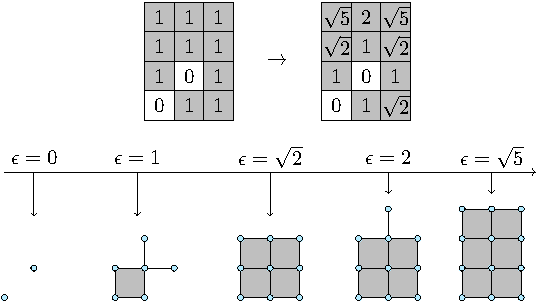
\includegraphics[scale=1]{cubicalfiltration.pdf}
    \caption{\label{edt} Transformation of a binary image into a filtration of cubical complexes based on the Euclidean Distance Transform.}
  \end{figure}

\end{example}

Our filtration on the volumes will describe the structure of the cornea starting at it the void surrounding it, then including the hollow shell which is its boundary, and then as the threshold increases the cubical complex will include more and more of the denser parts within the volume. An illustration of the thresholding at different values is seen in Figure \ref{thresh}.

\begin{figure}[ht]
  \centering
  \begin{subfigure}{.3 \linewidth}
  \centering
  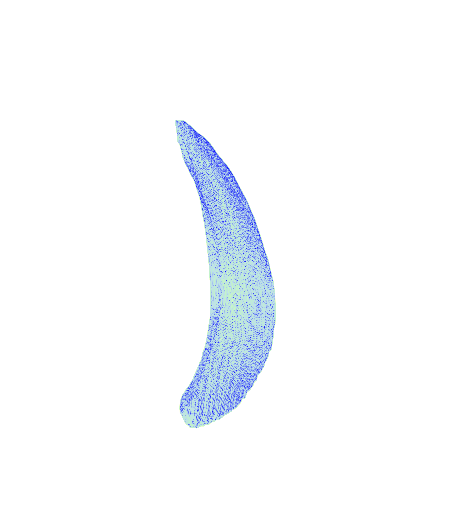
\includegraphics[scale=0.2]{eps2.png}
  \caption{$\epsilon < 2$}
  \end{subfigure}%
  \begin{subfigure}{.3 \linewidth}
  \centering
  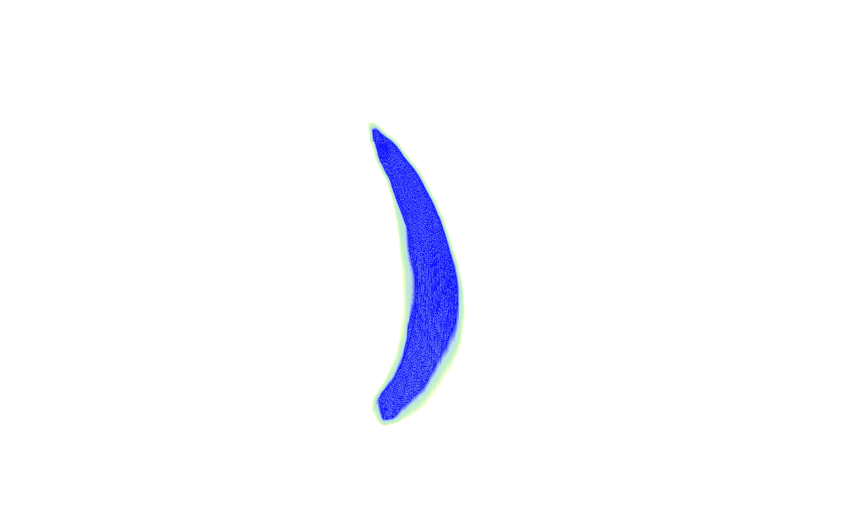
\includegraphics[scale=0.2]{eps10.png}
  \caption{$\epsilon < 10$}
  \end{subfigure}%
  \begin{subfigure}{.3 \linewidth}
  \centering
  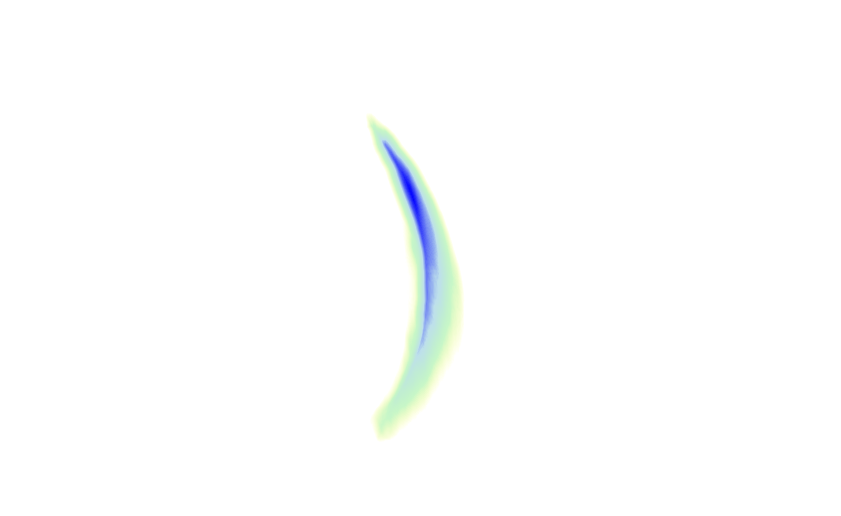
\includegraphics[scale=0.2]{eps100.png}
  \caption{$\epsilon < 100$}
  \end{subfigure}
  \caption{\label{thresh} EDT thresholding of BT\_77976. The pictures are rendered using by maximum projections, meaning that the value at each pixel is given by the maximum value in any of the voxels that a ray passes through. The colors are then mapped so that cooler colors indicate larger values relative to the other values in the rendering.}
\end{figure}

The resulting topological summaries we get are persistence diagrams. While these are in themselves interesting, in order to answer whether there is any relation between the size of an individual and the persistent homology of its cornea, we compute a distance matrix giving the distance of each sample to another.

Since we have a number of dimensions of homology to compare and two different distance metrics between persistence diagrams we get a total of 6 distance matrices. For each of these distance matrices, we divide them into two submatrices, one group consisting of the submatrix with entries from \textit{Bombus terrestris} and the other group consisting of all the other samples to act as a control group on the first.

Our hypothesis is that there is some relationship between the absolute difference in ITW between samples and the difference in persistent homology between the filtrations of cubical complexes constructed from the EDT of cornea volumes. But since different homology dimensions and metrics provide different summaries of the objects, we first need to figure out which one of them is most suited for our applications.

We determine which metric we will rely on by doing a so called \textbf{Mantel test} \cite[p. ~813]{mantel} of the distance matrix with respect to homology and the distance matrix with respect to ITW. A Mantel test is a non-parametric test of distance matrices, in which we compute the Spearman rank correlation of the two matrices under the null hypothesis that the matrices are uncorrelated. We can then derive a test statistic by permuting one of the matrices in both rows and columns and computing correlations for each such permutation.  The results of a Mantel test is a correlation coefficient indicating the strength of the correlation and $p$-value indicating how likely it is  that this coefficient would appear in a random permutation of one of the matrices.

We then perform clustering of the persistent homology distance matrix based on \textbf{hierarchical clustering}. It is a simple algorithm where we first consider each sample as its own cluster, and then group together clusters depending on the distance between them. The distance between two clusters is given as the minimum distance between any two samples between the two clusters. Our hope then is that the final clustering, based on persistent homology, reflects the ITW of the \textit{Bombus terrestris} samples.


\subsection{Results}
The Mantel tests in Table \ref{mantelc} reveal that the highest correlation is given by the bottleneck distance on $H_{2}$. Perhaps this is not too surprising, our objects are volumes and the most distinguishing aspects of volumes will be how they encode voids. Interestingly, the $H_{1}$ bottleneck distance matrix shows a very high $p$-value indicating that the largest distance between holes is not very telling in drawing a conclusion about correlation between size and persistent homology. This could be explained again by the fact that our object is a volume of a single connected component namely a cornea, and so any existence of holes will at best be local geometric information and at worst simply noise.

\begin{table}[h]
\begin{center}

\begin{tabular}{*6l}    \toprule
Group  & Metric  & $H_{1} \rho $  & $H_{1}$ p-value  & $H_{2} \rho$ & $H_{2}$ p-value  \\ \midrule
\textit{BT} & Bottleneck & $-0.069$ & $0.84$ & $0.86$ & $0.0083$\\
\textit{BT} & Wasserstein & $0.59 $ & $0.053 $ & $0.49$ & $0.080$\\
\textit{Others}& Bottleneck & $0.22$ & $0.030$ & $0.33$ & $0.0073$\\
\textit{Others}& Wasserstein & $0.23$ & $0.023$ & $0.26$ & $0.013$\\\bottomrule
 \hline
\end{tabular}
\end{center}

\caption{\label{mantelc} Table displaying the statistics computed in the Mantel test of the pairwise distances in different dimensions of persistent homology and the ITW for the species \textit{Bombus terrestris}. The symbol $\rho$ denotes the Spearman rank correlation coefficient computed between the two distance matrices. }
\end{table}

The $1$-Wasserstein metric does not provide a low enough $p$-value for us to draw any conclusions from the tests when it comes to \textit{Bombus terrestris}, this perhaps indicates that the sample size of the \textit{Bombus terrestris} submatrix is too small. It is possible that the more sensitive nature in the $1$-Wasserstein metric, since it records not only the largest differences in the persistence diagrams but all of them, makes it less robust to a smaller sample size.

Since the bottleneck distance on $H_{2}$ has a strong correlation with the ITW distance matrix we proceed with a hierarchical clustering on its distance matrix as seen in Figure \ref{h2b}. We see that there are two groups formed where one of the groups contains an additional cluster. The first group, which does not contain a subgroup, consists of two samples BT\_77967 and BT\_77976. These are the largest samples in terms of ITW and the remaining group contains two subgroups both in which the ITWs are smaller. It is worth repeating that this clustering is done without knowledge of the actual ITW, these clusterings are purely based on the bottleneck distance of the $H_{2}$ persistent homology and as such a differences here indicate differences based solely on the fact that their persistence diagrams differ.

\begin{figure}[ht]
  \centering
  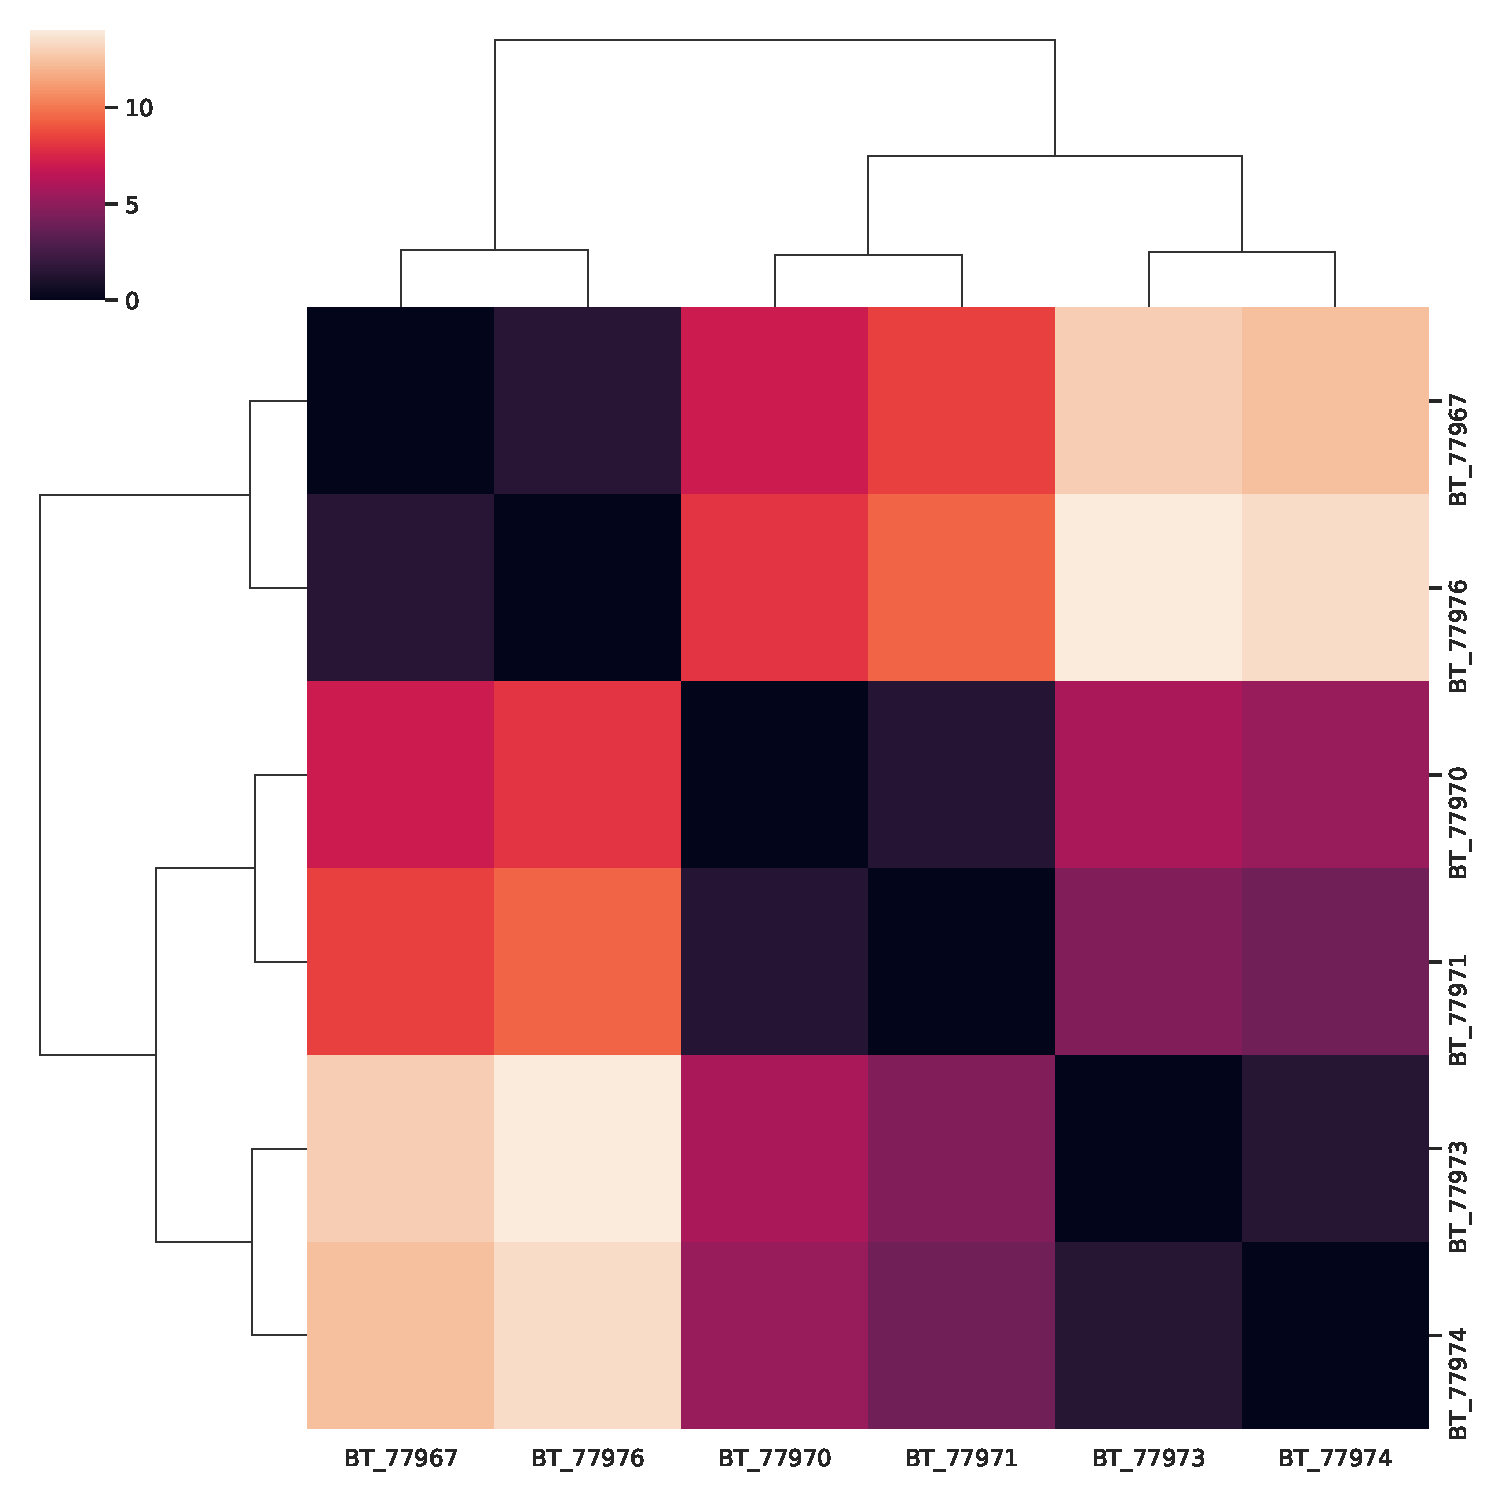
\includegraphics[scale=0.35]{clusters/bottleneck_h2_cluster.pdf}
  \caption{\label{h2b} Hierarchical single-link clustering of the bottleneck distance matrix derived from the persistent homologies of the \textit{Bombus terrestris} in $H_{2}$.}
\end{figure}

In order to further clarify in what way the persistence diagrams of the \textit{Bombus terrestris} are differing we can look at visualizations of the bijections done under the bottleneck distance and which pair of generators are the ones to determine the metric.

In Figure \ref{ingroup-matching} we see the matchings produced for the elements \textit{within} each of the identified clusters. We see that within the group the optimal matching always gives the largest distance as a matching between a point and the diagonal.

On the other hand, if we look at the distances from samples \textit{between} groups in Figure \ref{outgroup-matching} we see that there is one generator that is responsible for the bottleneck distance in all of these matchings. That is the longest living generator which is born at filtration value $0$. At filtration value $0$ the only voxels in the volume are the empty voxels constituting the background, which means that the void is left by the space where the cornea will be at a higher filtration value. As the filtration value increases the volume gets filled in with denser and denser parts of the cornea, but as seen in Figures \ref{ingroup-matching} and \ref{outgroup-matching} it lives for a long time before the cornea is entirely filled out. This difference in lifetime, which can somewhat be translated to the density of the cornea, appears to be the distinguishing factor between the three identified clusters of samples.

\begin{figure}[ht]
  \centering
  \begin{subfigure}{.49 \linewidth}
  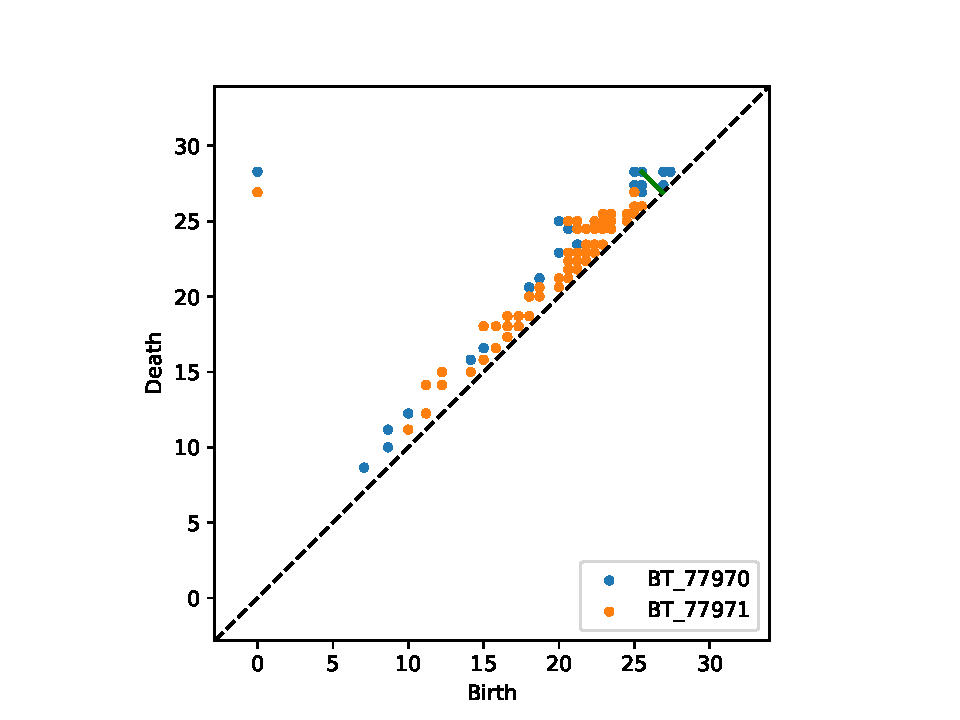
\includegraphics[scale=0.5]{matchings/77970-77971.pdf}
  \end{subfigure}%
  \begin{subfigure}{.49 \linewidth}
  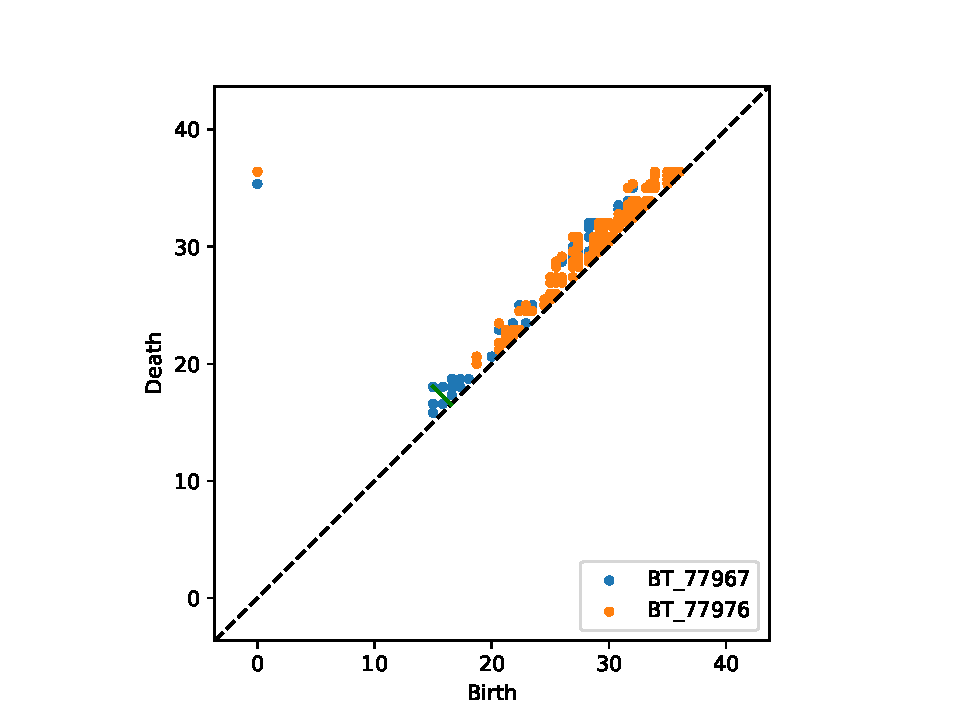
\includegraphics[scale=0.5]{matchings/77967-77976.pdf}
  \end{subfigure}
  \begin{subfigure}{.49 \linewidth}
  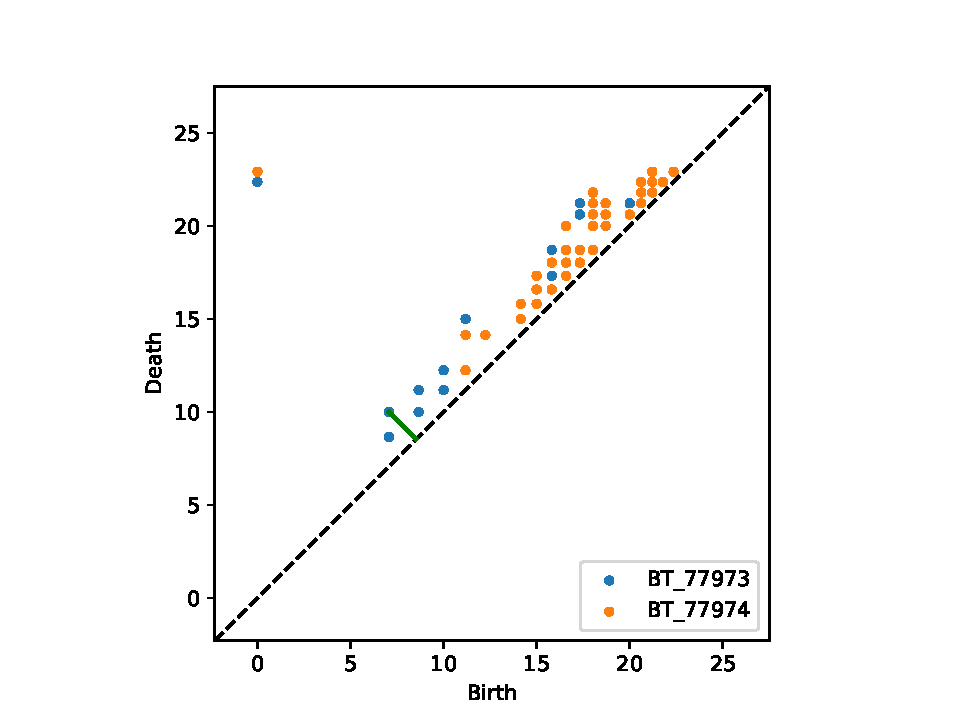
\includegraphics[scale=0.5]{matchings/77973-77974.pdf}
  \end{subfigure}
  \caption{\label{ingroup-matching} Visualisations of bottleneck distances within clusters on persistence diagrams of $H_{2}$.}
\end{figure}
\clearpage
\begin{figure}[ht]
  \centering
  \begin{subfigure}{.49 \linewidth}
  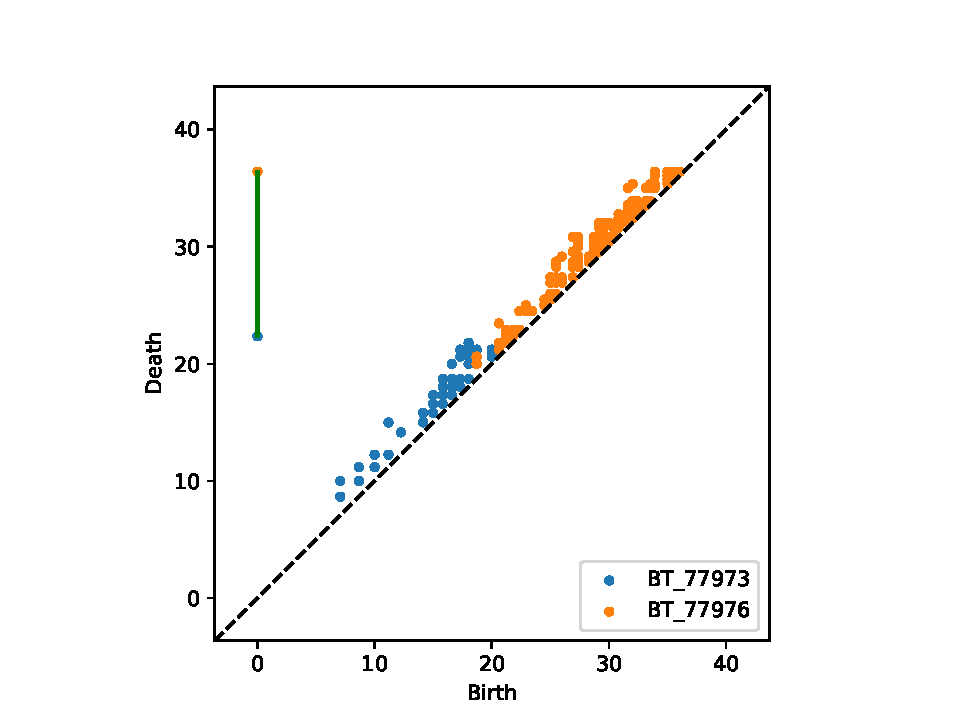
\includegraphics[scale=0.5]{matchings/77973-77976.pdf}
  \end{subfigure}%
  \begin{subfigure}{.49 \linewidth}
  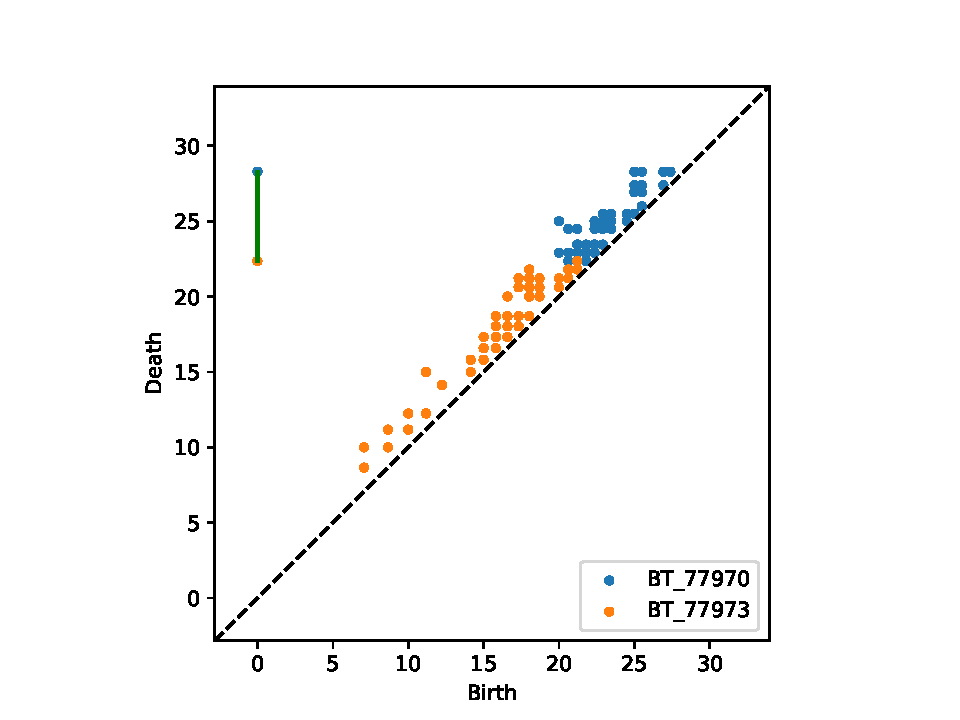
\includegraphics[scale=0.5]{matchings/77970-77973.pdf}
  \end{subfigure}
  \begin{subfigure}{.49 \linewidth}
  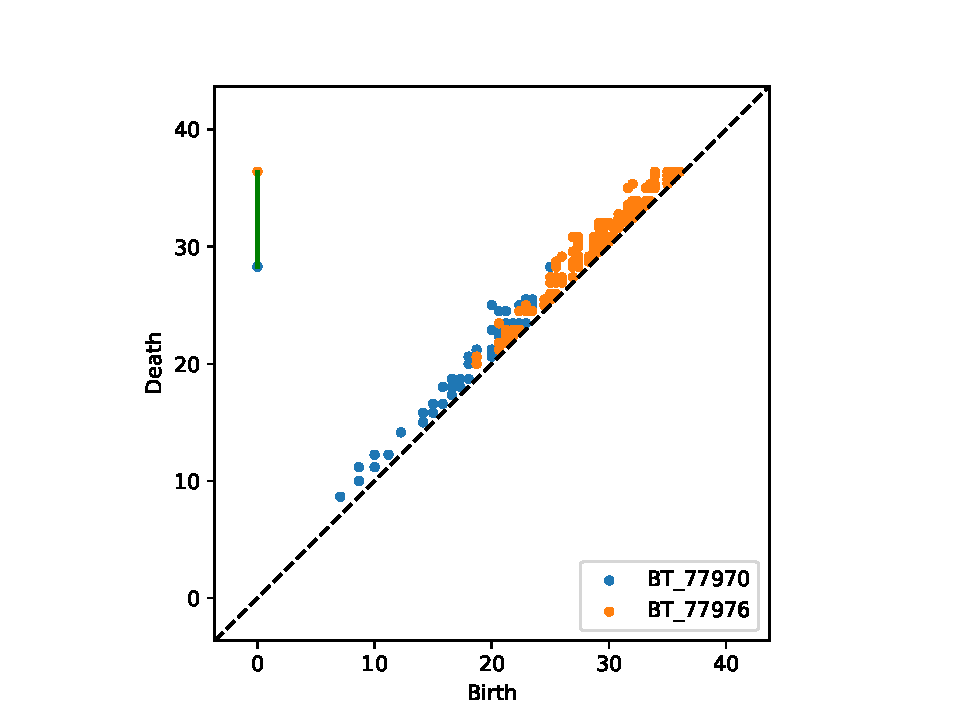
\includegraphics[scale=0.5]{matchings/77970-77976.pdf}
  \end{subfigure}
  \caption{\label{outgroup-matching} Visualisations of bottleneck distances between clusters on persistence diagrams of $H_{2}$.}
\end{figure}




While the purpose of this analysis is mostly to showcase persistent homology in the wild, these results  do support to the idea that different sized \textit{Bombus terrestris} do not only have larger eyes, but also that they are topologically different. Our clustering results on $H_{2}$ group the larger individuals together and we find a strong correlation with bottleneck distance in $H_{2}$ and ITW. Furthermore, we find that there is one generator born at the beginning of the filtration that is responsible for the ``bottleneck'' when comparing samples from the different clusters whereas within the same cluster other generators with much shorter lifetime are the contributors.
\clearpage
\section{The Simplicial Structure of the Striatum}
% The use of topological methods in order to understand brain networks is not new. There are a multitude of applications where persistent homology is used to overcome the problem of producing a graph from a set of a set sequence of connectivity maps by encoding all of them as a filtration. Traditional edge and vertex statistics have been generalized to simplices. Some other examples here.

There is much reason for considering simplicial complexes when it comes to networks related to the brain. An extensive field of study when it comes to network analysis of the brain are motifs, which at a high-level simply means a repeated pattern in a network which might have some form of semantic meaning to the network. Simplices capture such patterns at a micro-level through the connectivity of its faces. Furthermore, homology captures another type of patterns at a meso-level through cycles of simplices. Armed with persistent homology we arrive at a comprehensive summary of the network through the lens of the filtration of our choice.

In this analysis we follow \cite{reimann} by observing the high-dimensional simplicial structure of the brain by constructing a particular simplicial complex on the connectivity matrix of a synthetically generated microcircuit of the striatum as described in \cite{Hjorth202000671}, a part of the basal ganglia in the brain. By computing the resulting persistent homology we hope to discover distinguishing features of our network from a few selected control models. Furthermore, our aim is that this analysis serves as yet another example of the breadth of possible scenarios in which persistent homology is applicable outside the realm of theory. While we only investigate the mentioned microcircuit, our methodology is general enough for it to be applicable in any scenario where we data can be interpreted as directed graphs.

\subsection{Data}

Recall that a directed graph $G=\{V,E\}$ consists of a set of \textbf{vertices} $V$ and a set of \textbf{edges} $E$, where an edge is an ordered set $(v_{i},v_{j})$ for some vertices $v_{i},v_{j} \in V$. The \textbf{degree} of a vertex in a directed graph is the sum of the number of outgoing and incoming edges from and to the vertex.


In this case analysis our main object of study is a synthetic network based on the micro-circuitry of the striatum realized as a directed graph. The network is generated using empirical findings regarding connectivity between neurons, the morphology of cells and electrophysical properties, see \cite{Hjorth202000671} for further details. We compare this network to a three different models of directed graphs that all have different qualities common to networks of the brain.

\begin{definition}[{\cite{erdos}}]
The \textbf{Erdős–Rényi (ER) model} generates a directed graph through the choice of two parameters: the number of vertices $n$ and the number of edges $m$. The graph is then selected uniformly from the set of all graphs with $n$ vertices and $m$ edges.
\end{definition}

\begin{definition}[{\cite{strogatz}}]
The \textbf{Watts-Strogatz (WS)} model is parameterized by the number of vertices $n$, the average out-degree $m$ and a rewiring probability $p$. A directed graph is constructed by first creating a graph of $n$ vertices, such that for every vertex there is an outgoing edge to its $m$ closest neighbors modulo $n$, meaning that the graph is circular. Then finally each edge has a probability $p$ of being rewired to a different, uniformly selected, endpoint.
\end{definition}

\begin{definition}[{\cite{barabasi}}]
  The \textbf{Barabási–Albert (BA) model} is parameterized by the number of vertices $n$ and $m$, the average out-degree of each vertex. It is constructed by starting with the complete directed graph on $m$ vertices and successively adding vertices until there are $n$ vertices. For each new vertex $v_{i}$ we add an edge $\{v_{i},v_{j}\}$  with a probability of
  \[
    \frac{\deg(v_{j})}{\sum_{k} \deg(v_{k})}
  \]
  Hence, at each addition of a vertex an older vertex with a high degree has a higher chance of having its degree increased.
\end{definition}
ER can be considered the baseline model, since it is an arbitrary random graph among all possible graphs. WS is said to have \textbf{small-world properties}, which means that there are clusters of highly connected nodes and that the average path between two vertices is short. BA is said to be \textbf{scale-free} which means that most vertices have a low degree, but some ``hubs'' have a high degree. Both scale-free and small-world properties have been observed in brain networks \cite{SPORNS2004418}. Figure \ref{graphexamples} gives an example of each model generated with $100$ vertices.

In this analysis we compare the three models above with the synthetic network generated from the striatum, which we will refer to as ST. In Table \ref{graphmodels} we can see our choice parameters for the models and the resulting number of edges and vertices. For ER and WS our parameter choices were made to match the number of edges in ST. However, for the BA model we instead choose parameters in order to match the number of dimensions in the simplicial complex on ST as seen in Figure \ref{count50k}.
\begin{figure}[ht]
  \centering
  \begin{subfigure}{.33 \linewidth}
    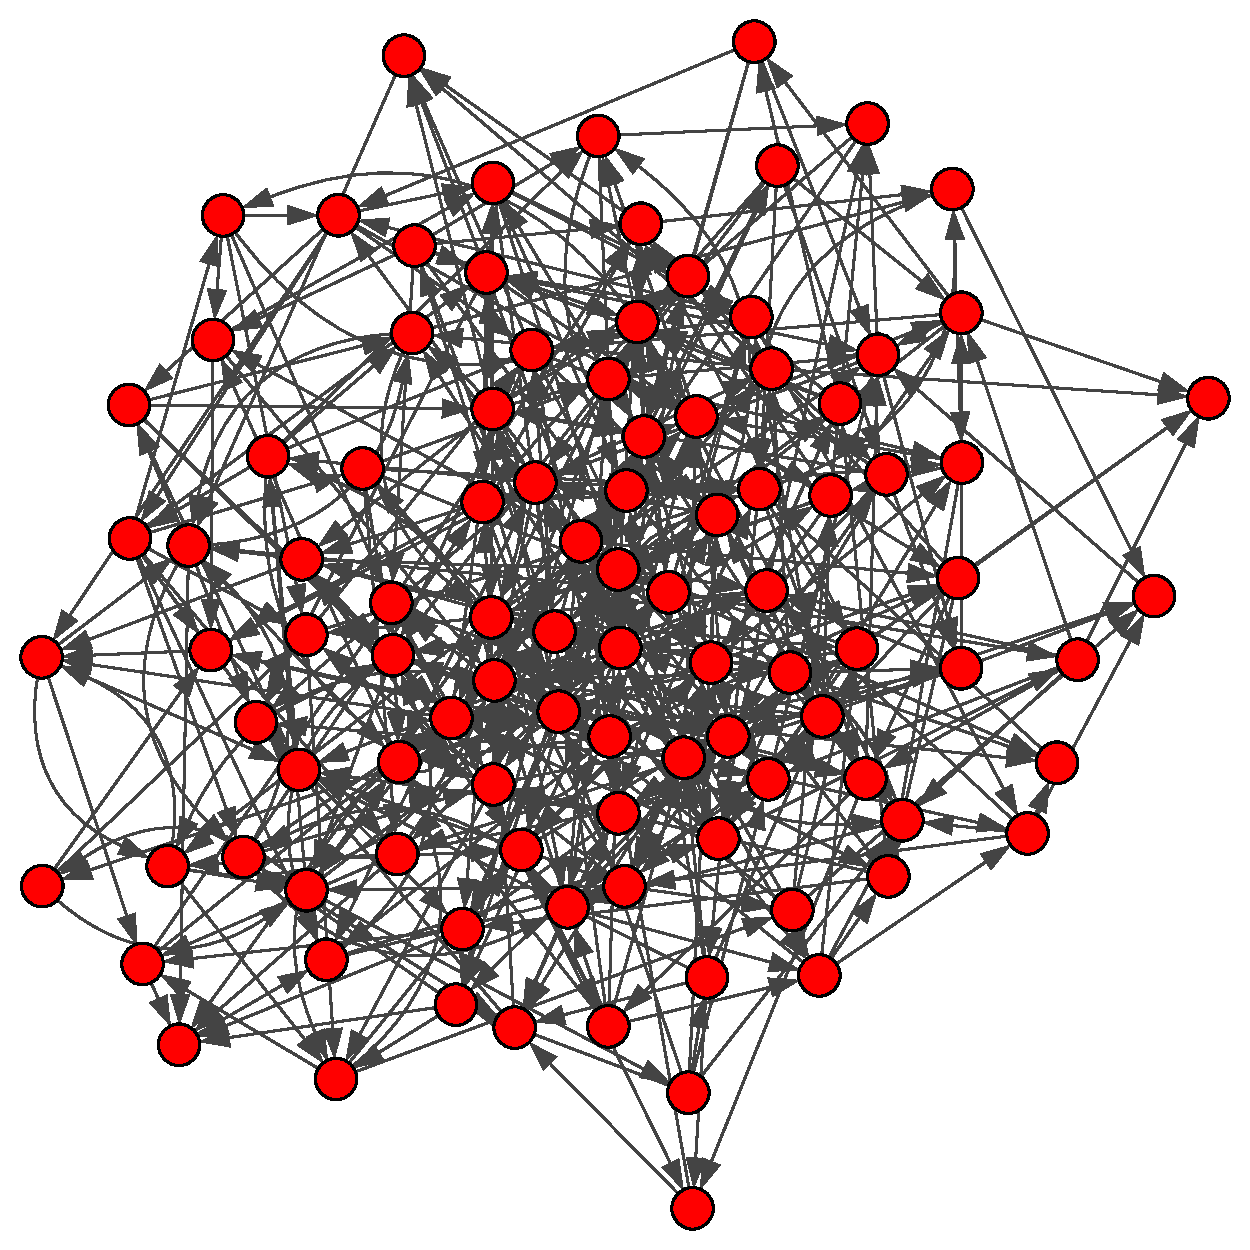
\includegraphics[scale=0.2]{random_graphs/erdos100v500e.pdf}
    \caption{Erdos-Rényi}
  \end{subfigure}%
  \begin{subfigure}{.33 \linewidth}

    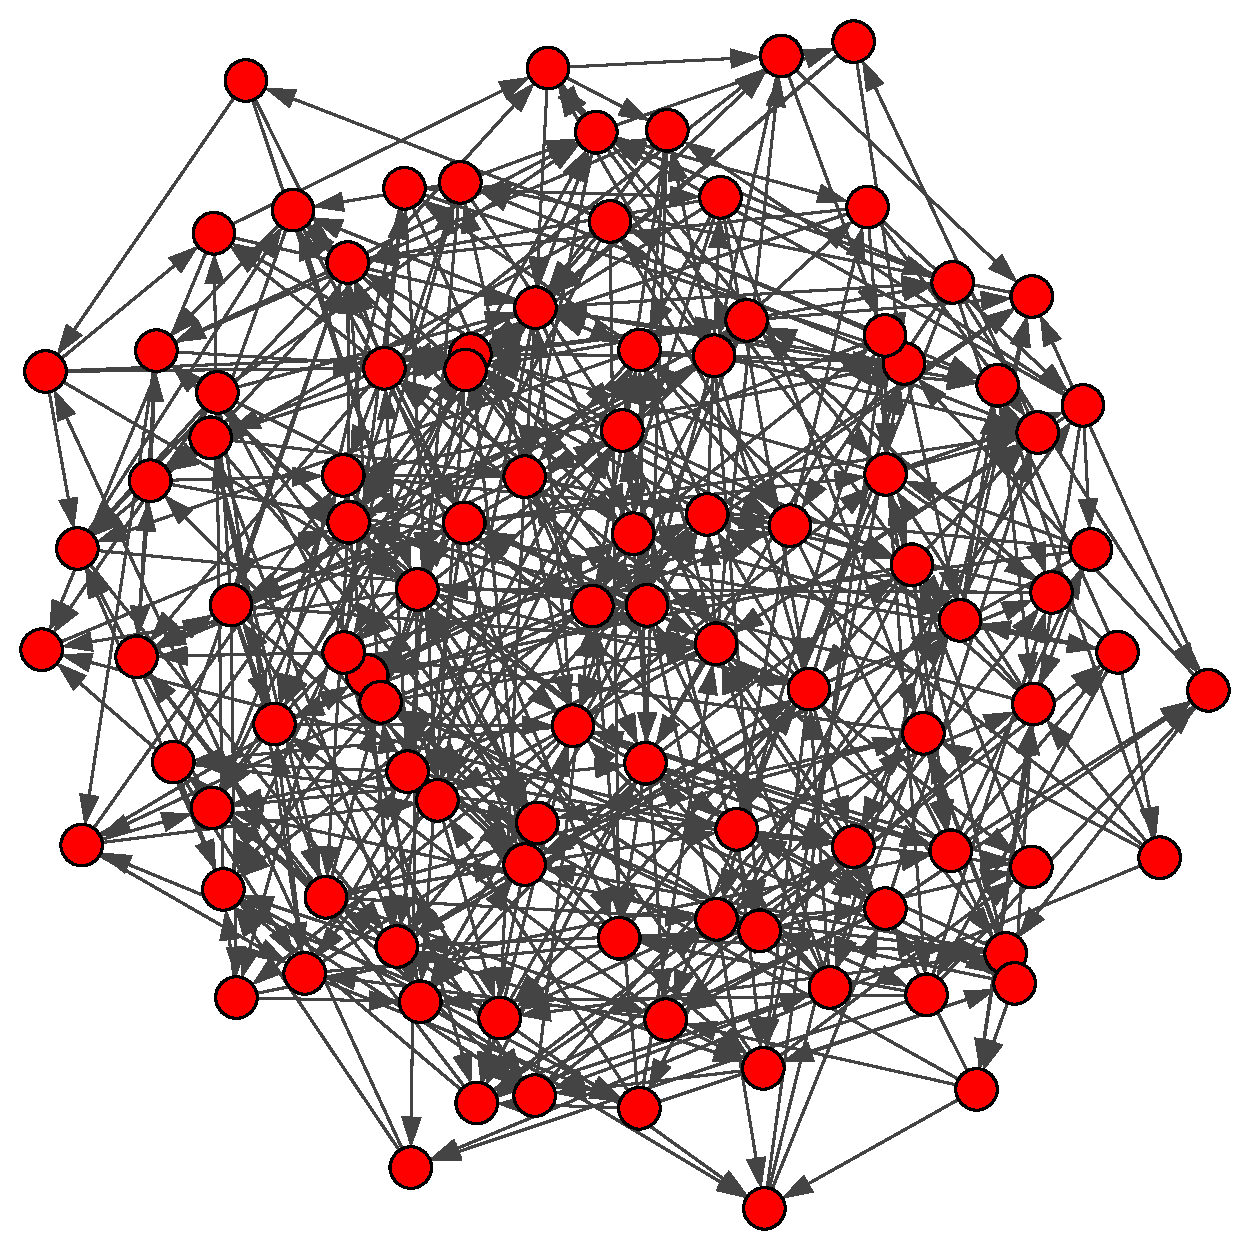
\includegraphics[scale=0.2]{random_graphs/strogatz100v5m05prob.pdf}
    \caption{Watts-Strogatz}
  \end{subfigure}%
  \begin{subfigure}{.33 \linewidth}

    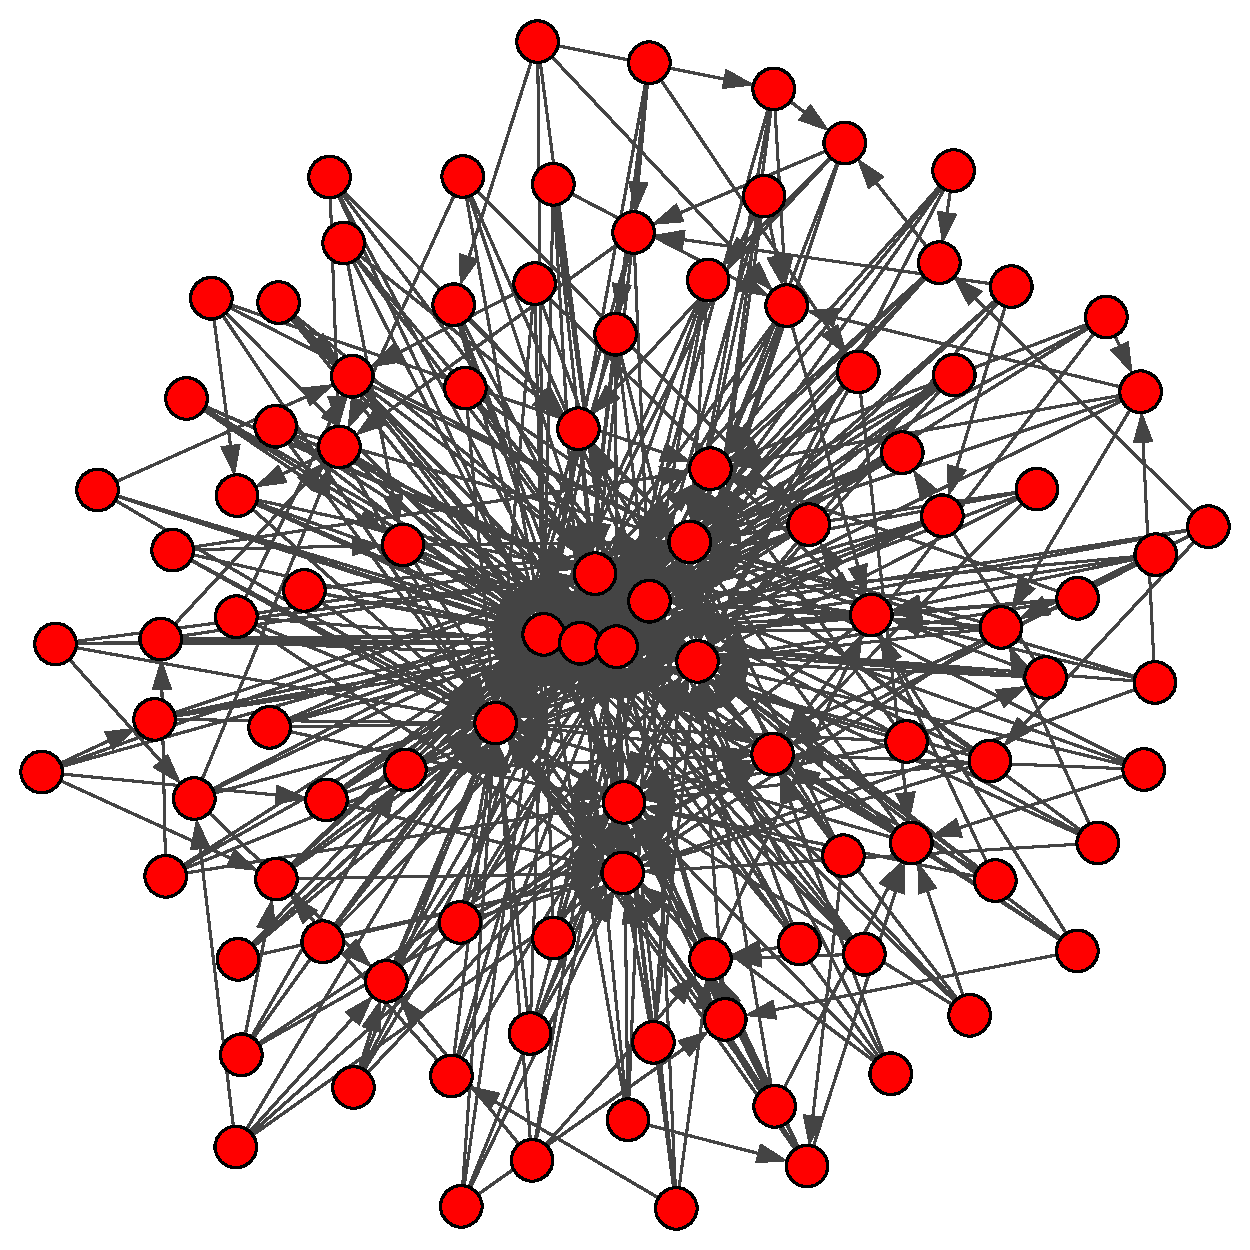
\includegraphics[scale=0.2]{random_graphs/barabasi100em5.pdf}
    \caption{Barabási-Albert}
  \end{subfigure}
  \caption{\label{graphexamples} An example of the ER, WS and BA models on 100 vertices.}
\end{figure}

\begin{table}[ht]
\centering
\begin{tabular}{*4l}    \toprule
  Network & Vertices & Edges & Parameters\\ \toprule
  ST & $50000$ & $12298074$  & - \\
  ER & $50000$ & $12298074$  & $n=50000, m=12298074$ \\
  WS & $50000$ & $12300000$  & $n=50000, m=247, p=0.5$  \\
  BA & $50000$ & $849864$ & $n=500000, m=17$
  \midrule
  \cr
  \bottomrule
\end{tabular}
\caption{\label{graphmodels} Breakdown of the ST, ER, WS and BA graphs compared in the analysis.}
\end{table}

\subsection{Methodology}
It is not entirely clear how we should define a simplicial complex on a \textit{directed} graph. The asymmetry is important as connections between neurons in the brain do not necessarily go both ways. While we could simply consider the network as a undirected graph by adding missing edges it is likely that important qualities of the network might be lost. There are a number of different ways to go about defining a similar complex on a directed graph. In our case we follow \cite{reimann} and construct something called the \textbf{directed flag complex} of a directed graph.

\begin{definition}[\cite{luetdigraph}]
  A \textbf{directed clique} is a directed graph $G=(V,E)$ such that every vertex has at least an outgoing or incoming edge to every other vertex in the graph. \end{definition}

Recall that an ordered simplicial complex as in Definition \ref{defordsimcomp} is given by an abstract simplicial complex together with a partial order that is total on each simplex. Hence, by taking a directed graph and introducing such a partial order on the vertices induced by the direction of each edge we can construct an ordered simplicial complex.

\begin{definition}[\cite{luetdigraph}]
  Let G=\{V,E\} be a directed graph. The \textbf{directed flag complex} dFl(G) is defined to be the simplicial complex whose $k$-simplices are all directed cliques with vertices $v_{0},\dots,v_{k}$ such that $\forall i: v_{i} \in V$
  and $\forall i,j: i < j \implies (v_{i}, v_{j}) \in E$. The vertices $v_{0}, v_{k}$ are called the source and the sink of a $k$-simplex.
\end{definition}

The directed flag complex is essentially the same construction given by the Vietoris-Rips complex where pairwise intersection is given by an edge. However, there are some notable difference due to the fact that the underlying graph is directed. The main difference is that we only create a simplex from cliques of simplices whose edges flow ``upwards'' in the order. This is because the total order on each simplex has to be respected in each of its faces. If we allowed for arbitrary directed cliques to be simplices the ordering would not be consistent. To see this, suppose that we have the directed simplices $[v_{0},v_{1}],[v_1,v_2],[v_{2},v_{0}]$ and $[v_{0},v_{1},v_{2}]$. Then the partial order of the vertices necessitates that both $v_{2} < v_{1}$ and $v_{1} > v_{2}$ which is a contradiction.

Since the directed flag complex is a simplicial complex homology is well-defined. However, when the partial order on the vertices of is \textit{not} a total order there are certain oddities to be aware of. For example, a reciprocal edge $v_{0} \leftrightarrow v_{1}$ in the underlying directed graph yields a generator of $H_{1}$ since the $1$-cycle $[v_{0},v_{1}]+[v_{1},v_{0}]$ cannot be the boundary of a $2$-simplex.

In Figure \ref{disimplex} we see how the left clique has a source and sink and thus defines a $3$-simplex in the directed flag complex, but the right clique has one edge going in the wrong direction, hence it is not a $3$-simplex.

% The $k$th chain module on a directed flag complex is defined in the exact same way as in Definition \ref{chainmodulesimp}. However, when the simplicial complex is constructed from a directed graph the partial order on the vertices is not necessarily total. As a result of this the chain complex has certain oddities like $[v_{0},v_{1}]+[v_{1},v_{0}]$ being a cycle whereas in the case of simplicial homology it would be a trivial chain TODO FIX THIS. In the context of a directed graph derived from the brain this makes sense: a connection between neurons is only one-way and the presence of a reciprocal edge indicates two different connections in both directions and thus is a cycle in its own right.

\begin{figure}[ht]
  \centering
  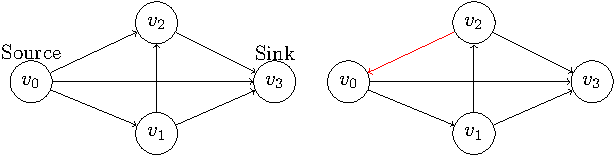
\includegraphics[]{./3simplex.pdf}
  \caption{\label{disimplex} Two directed cliques where the left clique does create a 3-simplex in the directed flag complex and the right clique does not.}
\end{figure}

We investigate the graphs ST, ER, WS, and BA in three different ways: the number of simplices in each dimension, their Betti numbers and their persistence diagrams.

For computing persistent homology, we need to define a filtration on the directed flag complexes.
We use a simple filtration function
\[
  f(\sigma) = \begin{cases}
    -\deg(\sigma) & \text{if } \dim(\sigma) = 0 \\
    \max_{\tau \text{ is a face of } \sigma} \{ f(\tau) \} & \text{if } \dim(\sigma) > 0
  \end{cases}
\] where we add vertices in descending order of degrees and their resulting higher-dimensional simplices whenever all their vertices have been included in the complex. The degree of the vertex indicates how central a vertex is to the graph, which means that the filtration will describe the network in its most basic building blocks and then add less and less important vertices.
\subsection{Results}
First we note the large number of simplices in ST as seen in Figure \ref{count50k}, where we find as much as over a hundred billion simplices in dimension $7,8$ and $9$. This phenomena was also observed in \cite{reimann}, however not of the same magnitude.  Furthermore, we see that the number of dimensions is significantly larger in ST compared to ER and WS. The graph BA was chosen so that its directed flag complex had the same dimension as ST's, but we see that the number of simplices in each dimension is notably lower. So while the BA model seems to capture the complexity of connectivity in ST it does not capture the magnitude. ER and WS present a lot fewer simplices and a lot fewer dimensions than ST. In this sense ER is the simplest model, but this is to be expected since it is a random graph we expect there to be less of simplicial complexity.

One thing that has to be mentioned is that the computation of homology and even more so persistent homology becomes extremely computationally expensive due to the number of simplices in ST. As seen in Section 3.3 reducing the boundary matrix in a dimension is at worst case given by a cubical amount of field operations in proportion to the number of simplices in one dimension above. Hence, computing something like $\beta_{7}$ for ST would involve a computation of the magnitude $10^{3 \cdot 11}$ field operations. Even worse, in practice computation persistent homology is not only affected by the number of simplices in the resulting simplicial complex, but also the number of simplicial complexes in the filtration. For this reason we only present persistence diagrams and Betti numbers for $H_{0},H_{1}$ and additionally the Betti number for $H_{2}$.

In Table \ref{bettis} we see that ST has a lower $\beta_{1}$ than any of the other graphs. Curiously, even though BA has a lot fewer edges it still has a higher Betti number in dimension 1. It is possible that the low amount of $1$-cycles is a feature that distinguishes brain networks from other types of networks, but no such result is presented in \cite{reimann} since $\beta_{1}$ was never computed due to computational limitations. If we turn to $\beta_{2}$ we see that $ST$ has the largest change from $\beta_{1}$, while the other graphs are pretty close to their $\beta_{1}$ however with a larger error. This dramatic increase from dimension 1 to dimension 2, both in Betti number and number of simplices, could also be seen as a feature of $ST$ compared to the other models. The distribution of simplices in Figure \ref{count50k} hints that this dramatic increase likely continues for several dimensions.

We see in Figure \ref{graphph} that ST is markedly different from all other models in terms of persistent homology. The persistence diagram of $BA$ is not very informative due to all of its vertices essentially having the same degree. However, WS and ER display similar persistence diagrams in which the distribution of holes is concentrated to a small interval of filtration steps from degree $500$ to degree $400$. In comparison, ST shows a much larger spread of both birth and death of holes, with some holes even being born or dying close to degree $0$.

To conclude, we have found that directed flag complex on $ST$ differs in several ways from the other three graphs: it has a much larger number of simplices in each dimension, it has simplices in high dimensions, it has lower $\beta_{1}$ than all models and lower $\beta_{2}$ than all models but BA. Furthermore, the persistence diagram of ST shows a distinct spread of the birth and death of generators of $H_{1}$, whereas for BA they are all born at the same time due to nature of the filtration and for ER and WS they are all restricted within a small interval of degrees.
%To interpret this, we have to remind ourselves of the definition of a $1$-dimensional hole in the context of a directed flag complex. It will be a cycle of edges such that there is no $2$-simplex, which is a triangle with a source and sink, including it. For example, a hole could look like this or like this both being valid holes, however it cannot look like this. This means that when a hole is killed, a vertex was added that gave rise to a vertex which turned the hole into a cycle. This only happens when
\begin{figure}[ht]
  \centering
  \begin{subfigure}{.49 \linewidth}
    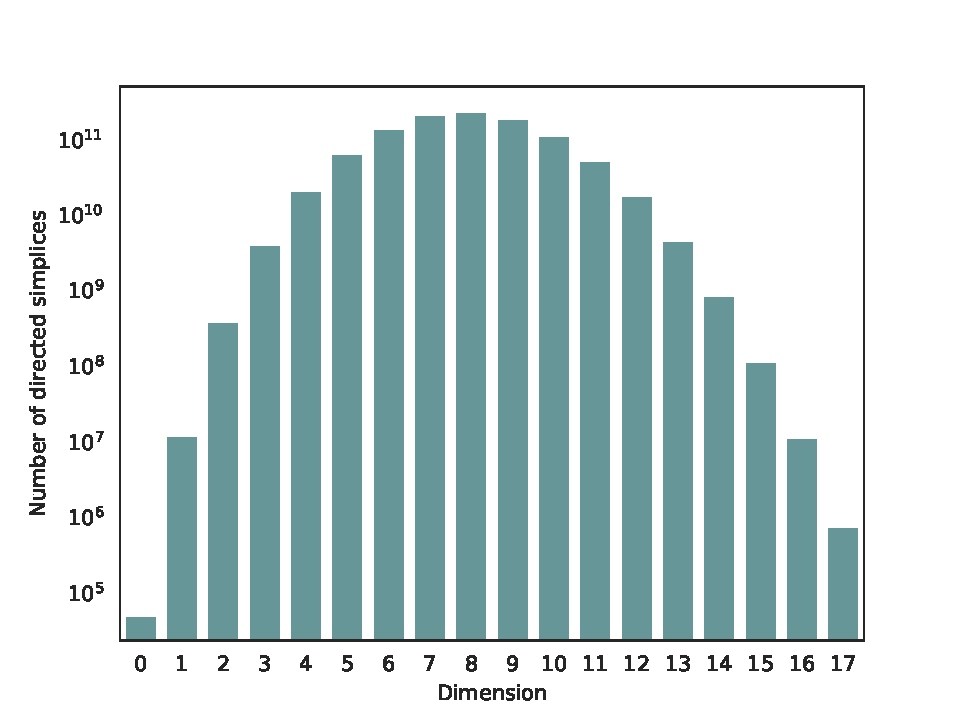
\includegraphics[scale=0.45]{./counts/real50k_count.pdf}
    \caption{ST}
  \end{subfigure}%
  \begin{subfigure}{.49 \linewidth}
    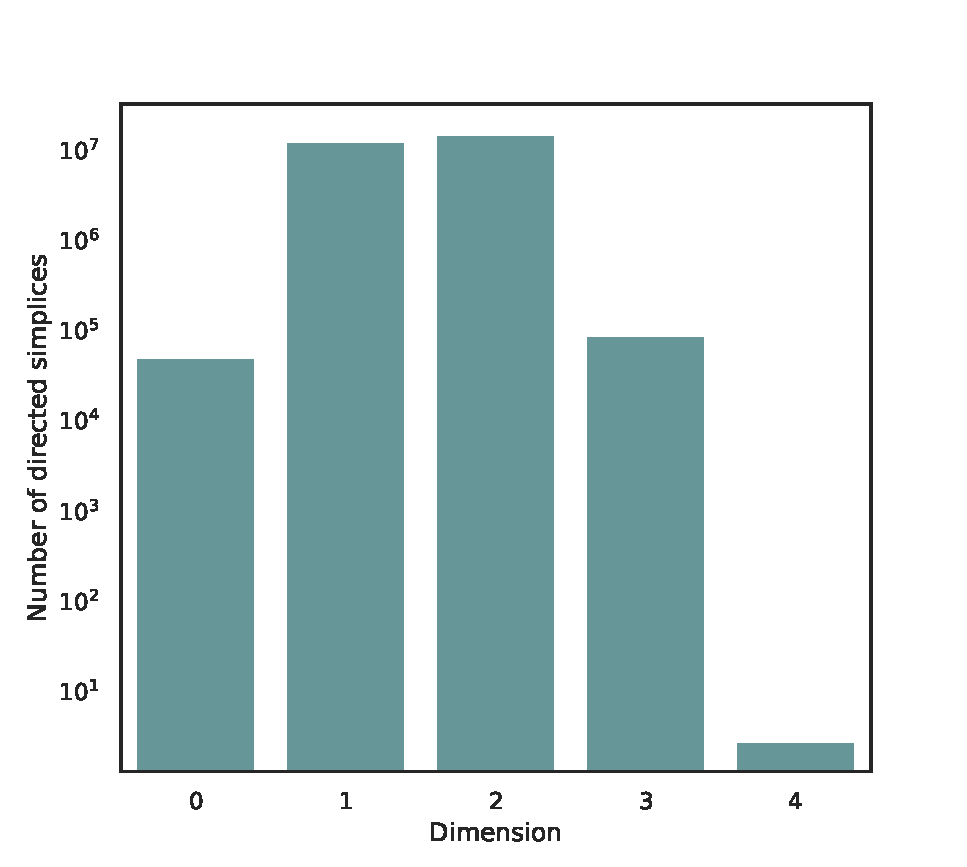
\includegraphics[scale=0.405]{./counts/random50k.pdf}
    \caption{ER}
  \end{subfigure}
  \begin{subfigure}{.45 \linewidth}
    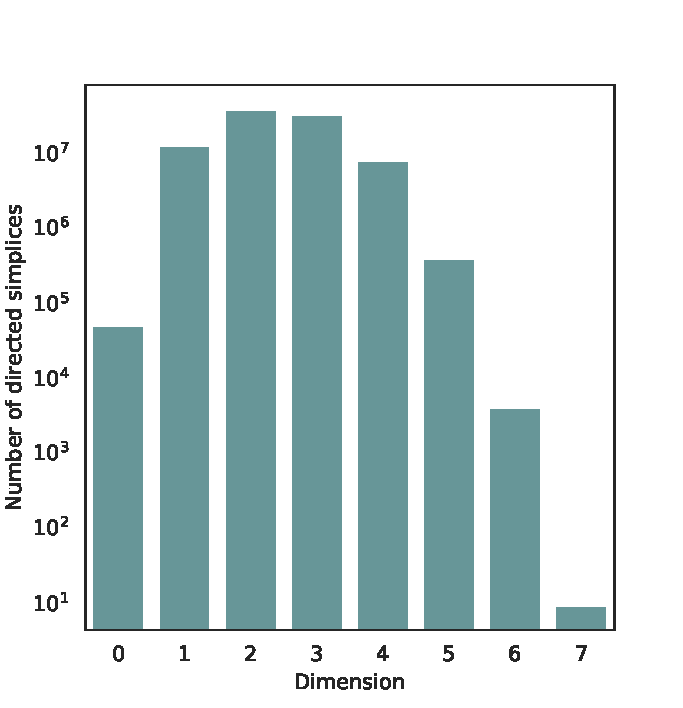
\includegraphics[scale=0.49]{./counts/random50k_ws_count.pdf}
    \caption{WS}
  \end{subfigure}
  \begin{subfigure}{.49 \linewidth}
    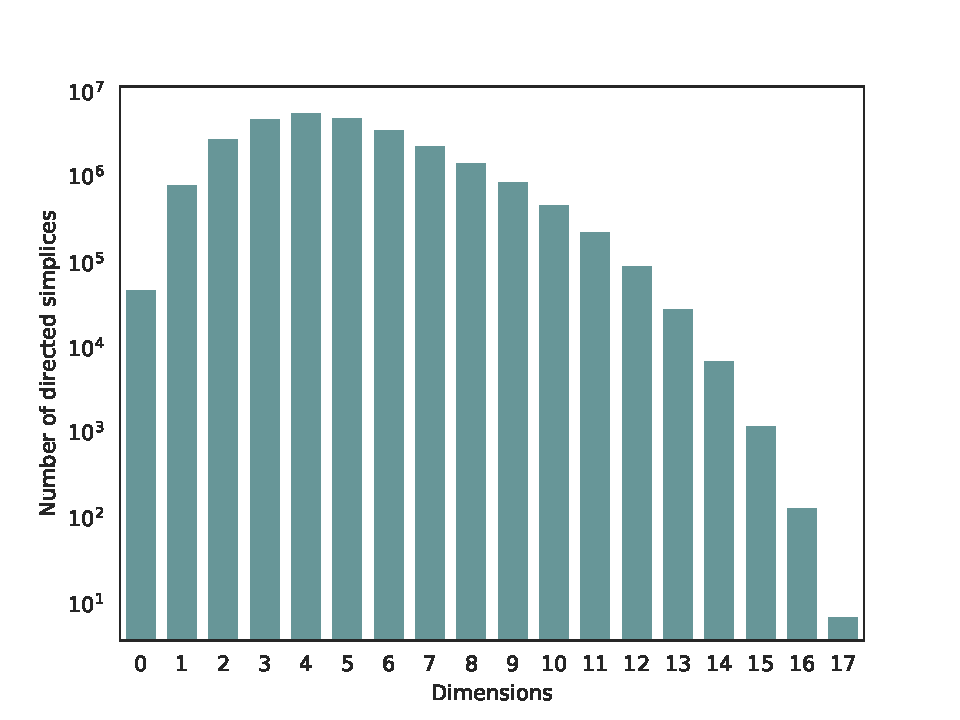
\includegraphics[scale=0.49]{./counts/random50k_ba_count.pdf}
    \caption{BA}
  \end{subfigure}
  \caption{\label{count50k}The total number of simplices in each dimension for the directed flag complex on ST, ER, WS and BA. For ER, WS and BA the counts are the result of the mean number of simplices in each dimension over 100 computations.}
\end{figure}
\begin{table}[ht]
\centering
\begin{tabular}{*4l}    \toprule
  Network & $\beta_{1} $  & $\beta_{2}$  & Computations \\ \toprule
  ST &   $5128 \pm 1219$ & $293013 \pm 79867$ & 1 \\
  ER &  $369770.18 \pm 687.69$ & $3470380.91 \pm 2774.23$ & 100 \\
  WS & $334754.93 \pm 625.38$ & $3756595.22 \pm 3709.97$ & 100 \\
  BA &  $11982.51 \pm 956.18$ & $12946.77  \pm 1734.00$ & 100
  \midrule
  \\
  \bottomrule
\end{tabular}
\caption{\label{bettis} Table over the first and second Betti numbers for the graphs ST, ER, WS and BA. The computation column denotes the number of instances of the model over which the result was averaged, hence the Betti numbers are given by an average value and its standard deviation. For ST the approximation seen in \cite{luetdigraph} was used in order to reduce computational time in which some columns were not reduced to Smith normal form. Every such non-reduced column can at most subtract or add one Betti number.}
\end{table}

\begin{figure}[ht]
  \centering

  \begin{subfigure}{.49 \linewidth}
    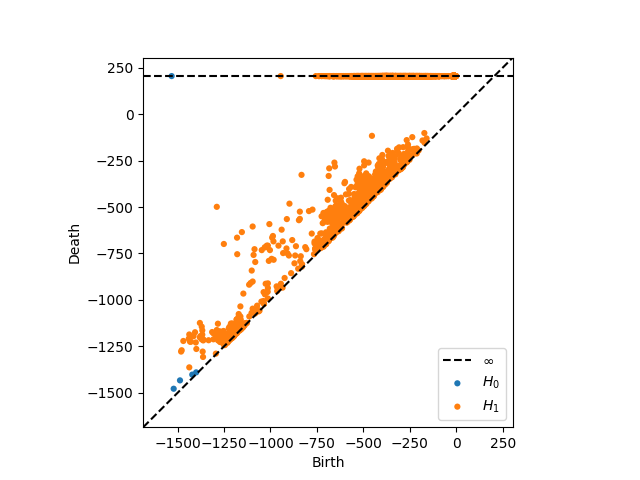
\includegraphics[scale=0.49]{./graph_phs/ST.png}
    \caption{ST}
  \end{subfigure}%
  \begin{subfigure}{.49 \linewidth}
    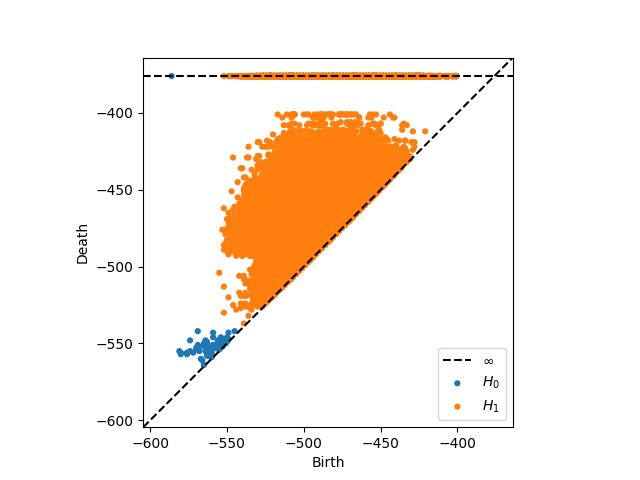
\includegraphics[scale=0.49]{./graph_phs/ER.png}
    \caption{ER}
  \end{subfigure}
  \begin{subfigure}{.49 \linewidth}
    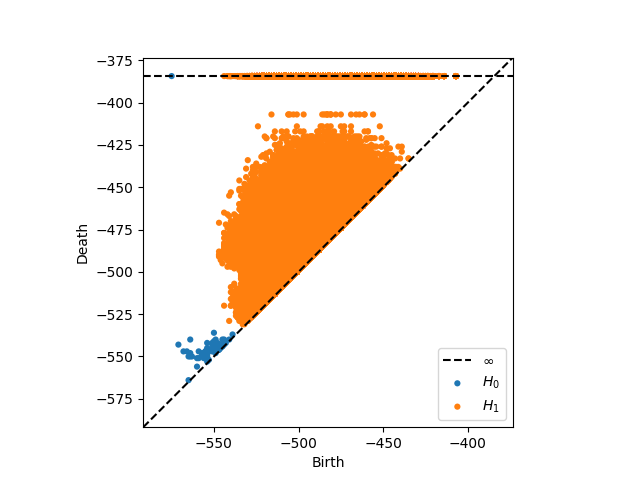
\includegraphics[scale=0.49]{./graph_phs/WG.png}
    \caption{WS}
  \end{subfigure}
  \begin{subfigure}{.49 \linewidth}
    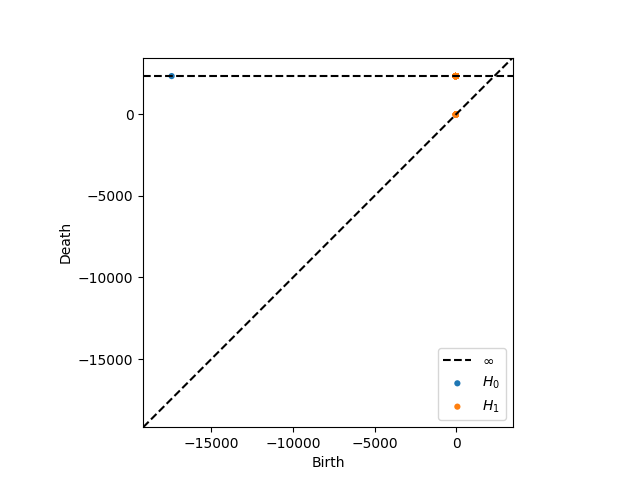
\includegraphics[scale=0.49]{./graph_phs/BA.png}
    \caption{BA}
  \end{subfigure}
  \caption{\label{graphph} Persistence diagrams over $H_{0}$ and $H_{1}$ for ST,ER,WS and BA given by inclusion of vertices and their resulting higher order simplices in the negative order of their degrees.}
\end{figure}

%%% Local Variables:
%%% mode: latex
%%% TeX-master: "thesis.tex"
%%% End:
